\documentclass[conference]{IEEEtran}
\IEEEoverridecommandlockouts
% The preceding line is only needed to identify funding in the first footnote. If that is unneeded, please comment it out.
\usepackage{cite}
\usepackage{amsmath,amssymb,amsfonts}
\usepackage{algorithmic}
\usepackage{graphicx}
\usepackage{textcomp}
\usepackage{xcolor}
\usepackage{float}
\usepackage{minted}
\usepackage{cuted}%%\stripsep-3pt

\def\BibTeX{{\rm B\kern-.05em{\sc i\kern-.025em b}\kern-.08em
    T\kern-.1667em\lower.7ex\hbox{E}\kern-.125emX}}
\begin{document}

\title{Github Data Analysis\\
{\small Wide Project Proposal}
}

\author{
\IEEEauthorblockN{YUAN Yingzhe}
\IEEEauthorblockA{\textit{Computer Science and Enigeering} \\
\textit{HKUST}\\
Hongkong, China }
\and
\IEEEauthorblockN{GUO Jiong}
\IEEEauthorblockA{\textit{Computer Science and Enigeering} \\
\textit{HKUST}\\
Hongkong, China}
}

\maketitle

\begin{abstract}
    GitHub have huge user group. Every moment there are hundreds of activities happen. To analyze the GitHub data continually, we use some opensource big data component such as Hadoop, spark, hive to construct a GitHub data processing framework, which aims at handling massive activity records and analyze data to find out patterns of users, repositories and languages. Using python crawler to get data from GitHub. By different data processing skills, the data is transport by certain channel to provide the downstream usage. Building the data warehouse base on the structure and content of the data and make three layers of the data warehouse. By spark, making data analyzation and store the result in the relational database. Finally present the graph and table on the dashboard.
\end{abstract}

% \begin{IEEEkeywords}
% Github, Spark, Data Analysis, Data Mining
% \end{IEEEkeywords}


\section{Introduction}

Github is an open source platform for developers to share their codes and collaborate with others. In this project, we will use spark to construct a real-time processing framework, which aims at handling massive activity records and analyze data to find out patterns of users, repositories and languages. 

\section{Dataset}

All the data we will use in this project are from Github. There is not an existing complete dataset to get enough well-structured data for our project, so we need to collect data and preprocess by ourselves. In this section, we will illustrate why we choose Github's data and what the data sources are.

\subsection{Why Github}
Github is the largest developer community and the largest platform for developers to share their codes and collaborate with others in the world. By analyzing the data from Github, we can get some insights about the development of open source projects, the development of programming languages, and the development of the developer community.



\subsection{Source I: Open API}
Github provides a series of open API for developers to access most of the informations on Github. This 'Github REST API\cite{ghapi}' is mainly used for creating integrations, retrieve data, and automate workflows, but we can use it to query specific data needed for our project.

There are mainly two main areas of data:

\begin{itemize}
    \item \textbf{Users:} Basic open informations of user, such as id, name, email, following users, repositories owned, etc.
    \item \textbf{repositories:} Basic information of public repositories, such as id, name, owner, description, stars etc.
\end{itemize}

We will provide some examples results of API query in Appendix\ref{a-ghrest}.

There are limits of current official REST API:
\begin{itemize}
    \item Some need authentication, which means we need to provide a valid token to access the data.
    \item Some API cannot be called too frequently, which means we need to wait for a while before we can call it again.
    \item Most of API need an \textbf{\textit{id}} as its query parameter, so we need to get the id first before we can query the data, which means we need to construct a massive id list.
\end{itemize}

After considering the above limitations, we decide to use the Github Archive\cite{gha} as our main data source and use the REST API to get some additional data or search some specific content.


\subsection{Source II: Github Archive}

\textit{GH Archive\cite{gha} is a project to record the public GitHub timeline, archive it, and make it easily accessible for further analysis.} In fact, it also based on Github's Open API, while only use the \textbf{activity} API:



\begin{minted}[breaklines,breakautoindent,mathescape,linenos,numbersep=1pt,frame=lines,framesep=2mm,fontsize=\footnotesize,baselinestretch =1,style=emacs]{python}
    https://api.github.com/events
\end{minted}


\textbf{GH Archive} will crawl github's activity data in real time and sort them as json file in order of when they occurred. Activity archives are available starting from 2011-02-12, and are updated amost half day, so the total size of data is \textbf{TB} level. 

Considering too large size of the data and the the earlist data using a different format, we will only use the latest part of them. In fact, the current amount data of data in an hour is about 700MB, so the latest data is surely enough for our project. The corresponding compression packages with specific time can be downloaded easily, and the minimal time interval of packages is one hour. 

\begin{figure}[H]
    \centering
    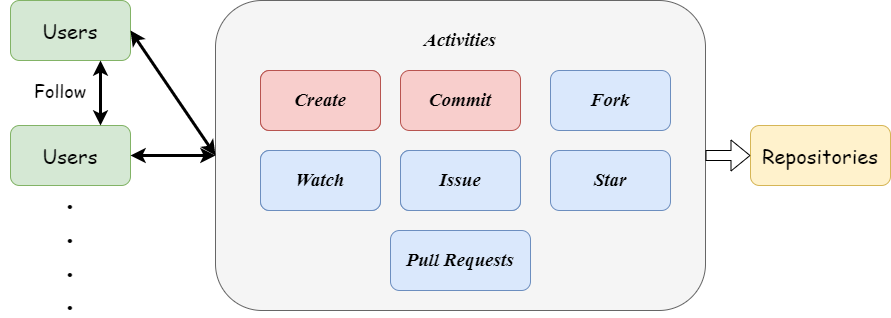
\includegraphics[width=0.45\textwidth]{./pic/github.png}
    \caption{This figure shows relation between user and repository and basic activities.}
    \label{fig:github}
\end{figure}


The archieved activity data contains almost all 20+ event types provided by Github, which ranges from new commits and fork events, to adding members to a project. We will only pay attention to some key event type, such as \textit{commit}, \textit{create}, etc.

We will give some example of the data format in Appendix\ref{a-gha}.


\subsection{Summary}
Based on almost all activity record, Github's Open API can help us to get almost all related information. For example, from \textbf{GH archive}, we know user a push a commit at 12:00 in repository A, then we can get almost all details of a and A by calling Github's API.








\section{Task}

Github has provided some basic data aggregation for user to explore. For example, in \textbf{\textit{Trending\cite{ghtrending}}}, Github shows the most popular repositories in the specific time range, language and spoken language. In \textbf{\textit{Topics\cite{ghtopics}}}, Github shows repositories' topics according to tags of repositories. However, these data analysis are very basic and not wide to cover most of the information in Github.

In this project, we will use spark to construct a real-time processing framework, which aims at handling massive activity records and analyze data to give a more comprehensive analysis of Github.

There are main tasks in this project:

\subsection{Data Preprocess}

\begin{enumerate}
    \item \textbf{Collect} data. Crawl Github Archive\cite{gha} and use Github API\cite{ghapi} to jointly query more detailed information about activities according to indices in Github Archive. Though Github Archive update several times a day, we will simulate it to a real-time stream to process data in real-time. 
    \item \textbf{Preprocess} data by Spark. For complete each json record, split it into several parts, filter useful parts and store them in different tables.
    \item Data \textbf{Persistence}. Design different schema and construct key meta tables to store necessary information, statistics result or some data not easily obtained directly.
\end{enumerate}

\subsection{Data Analysis}

\begin{enumerate}
    \item \textbf{Statistics}. We wiil try to construct a dashboard to show some basic statistics of Github, such as the repository with the highest frequency of commits, the most frequently commits time period, etc.
\end{enumerate}


\subsection{Data Visualization}
\begin{enumerate}
    \item \textbf{Dashboard}. We will try to construct a dashboard to watch the process of data process and show the results of data analysis by deploying a webpage.
    \item \textbf{Interaction}. We will try to make the dashboard interactive, such as users can choose the time range of data to analyze, or choose the language to analyze, etc. Results of corresponding process not only comes from persistant database, but also from real-time stream produced by Spark.
\end{enumerate}








\section{System Framework}

\subsection{Cloud Server Configuration}

\subsubsection{Memory and Cores}

The system architecture contains many components. The metastore of hive is deployed on mysql, so that hive can be used by multiple users. Therefore, we need to choose a server with large memory to accommodate all components. Considering the system requirements, we choose a server with 4 cores and 16G memory.


\subsubsection{Server Type}

Our task is to build a data analysis service platform that continuously obtains log information and do data analyze jobs. We chose preemptible instances because of their relatively low price. And we have developed a set of fully automated scripts to deploy the cluster, so that if the server needs to be released unexpectedly, the service can be easily deployed to the newly created server.


\begin{figure}[H]
    \centering
    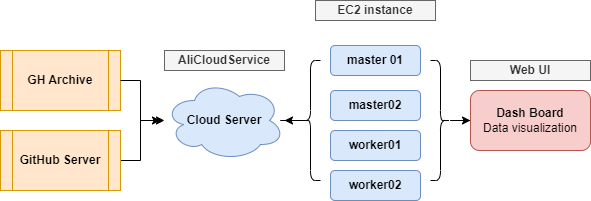
\includegraphics[width=0.45\textwidth]{./pic/server.png}
    \caption{A figure shows types of servers}
    \label{fig:server}
\end{figure}



\subsubsection{Final Cluster Choice}


For the final cluster, we use 4 server, which are named as \textit{master01}, \textit{master02}, \textit{worker01} and \textit{worker02}. Different server played as different character in the cluster.


The Server details information:
\begin{itemize}
    \item Instance type: Preemptible Instance
    \item Specifications: 4v CPU 16 GiB (I/O Optimized)
    \item Storage: 40GiB Cloud disk for each server
    \item Network: 100Mbps
\end{itemize}



\begin{figure}[H]
    \centering
    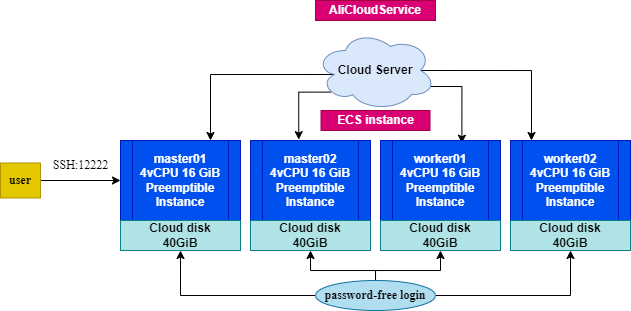
\includegraphics[width=0.45\textwidth]{./pic/server-info.png}
    \caption{A figure shows details configuration of clusters}
    \label{fig:server-info}
\end{figure}



\subsubsection{Auto Configuration}
Preemptive servers may be automatically released for lack of resources by Aliyun, so we need to purchase new computation instances, deploy the original big data system quickly and recover data collected when that worst situation happens. Based on this requirement, we have implemented a complete automatic configuration shell script, so that only one script need to be executed on any one single node to complete the environment configuration and deployment of the whole cluster, which greatly improves the efficiency of the cluster deployment and reduces the workload of the administrator.


\begin{figure}[H]
    \centering
    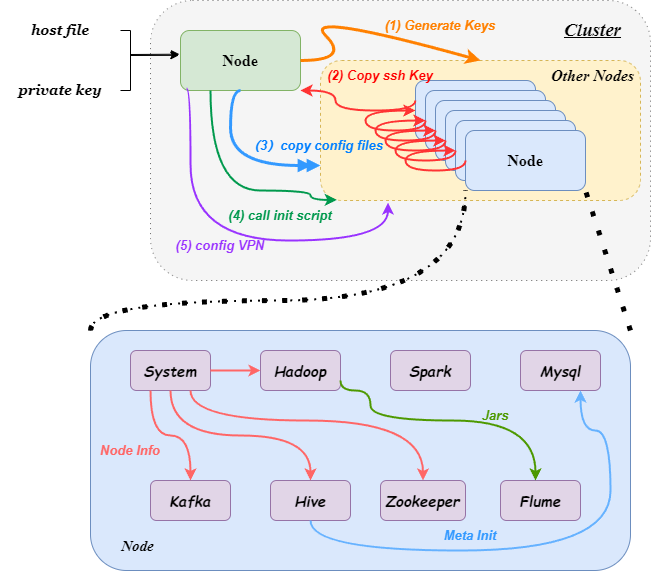
\includegraphics[width=0.5\textwidth]{./pic/autoconfig.png}
    \caption{A figure shows the control flow of auto configuration}
    \label{fig:autoconfig}
\end{figure}

\paragraph*{Cluster}
For the whole cluster:
\begin{enumerate}
    \item Upload private key (for log in server initially) and host file (record the ip and name of all nodes) to any one nodes \textit{A}.
    \item Execute autoconfig shell script, which will do the following things one by one:
    \begin{enumerate}
        \item Require each node to generate a new ssh key pair and update sshd configuration.
        \item Each node broadcasts its own public key to all other nodes for password-free login. Then only use the new own key to log in to other nodes after that.
        \item Synchronize all necessary config files of components(hadoop, spark, etc) from \textit{A} to all other nodes.
        \item Execture the installation script on each node's background.
        \item After the installation is complete, all nodes need to config a VPN proxy to access the outer Internet for downloading Github data.
    \end{enumerate}
\end{enumerate}

All big data components will be installed when installation script is executed. The installation script will do the following things one by one on each node:
\begin{enumerate}
    \item Install system software, update system environment variables and create necessary directories.
    \item Modify configuration files of each component according to the node's role and special information, such as zookeepers'id, etc.
    \item Download and install all components one by one, and copy the configuration files to the corresponding location.
    \item Copy essential \textbf{\textit{Jars}} of hadoop and spark to other components' \textit{lib} directory, such as flume, which is used for ensure consistence of the version of all components to avoid potential problems.
    \item MySQL will be installed on \textit{worker02}, modify access authority, and init database schema. The JDBC driver will be installed on all nodes.
    \item Init hive metastore database on \textit{worker02}. The hive schema will be stored in MySQL.
\end{enumerate}



\subsubsection{Security Control}    
After deployment, servers are frequently attacked from unknown sources, including DDoS, mining viruses, worms, and remote controlling, which causes the extremely high CPU usage, high disk IO, and unable to access the server. Killing processes, resetting servers, and recollecting data took up over 40\% of our time


Although it has been observed that the behavior after entering the server is to inject code into the process, it is not clear by what means the server was successfully accessed and permissions obtained. We have taken the following steps to try to avoid being attacked:

\begin{itemize}
    \item \textbf{Change the default port of sshd}: The default port of sshd is 22, which is the most frequently attacked port. We changed the port to 2222, which greatly reduced the number of attacks.
    \item \textbf{Only allow strict key login}: Some instruction of automated configuration steps need to be provided password, we generated a random length of 40 characters password by openssl and only use it once. After the configuration is complete, the password will be deleted, and all communication will be based on the rsa key.
    \item \textbf{Close unnecessary ports}: We only preserve port for ssh login and data visualization for external network access, and other ports of big data components are only open to the internal network.
    \item \textbf{Install anti-virus software}: We installed \textit{ClamAV} on each node to scan the system periodically.
\end{itemize}

All above measures cannot completely prevent attacks, and we believe there is an unknown vulnerability. The corresponding logs are in the appendix.




\subsection{System Architecture}
Our goal is to build a distributed file system and computing analysis system based on cloud servers. After identifying the servers and clusters, we need to decide where to deploy the components and how data will flow between the different components within the architecture.



\subsubsection{Technology selection}

Considering our needs, we need to build a distributed file system and distributed computing system for continuously input log information, and need to store related information such as users and warehouses. So we choose the most commonly used technology in the field of big data: Hadoop architecture. Considering the data form we need, we use hive to store the data as hive tables. For faster analysis, we use spark for distributed computing and analysis. According to the main thread, we add more components to it to maintain the continuous operation of the whole system.



\subsubsection{Deployment}

\begin{figure}[H]
    \centering
    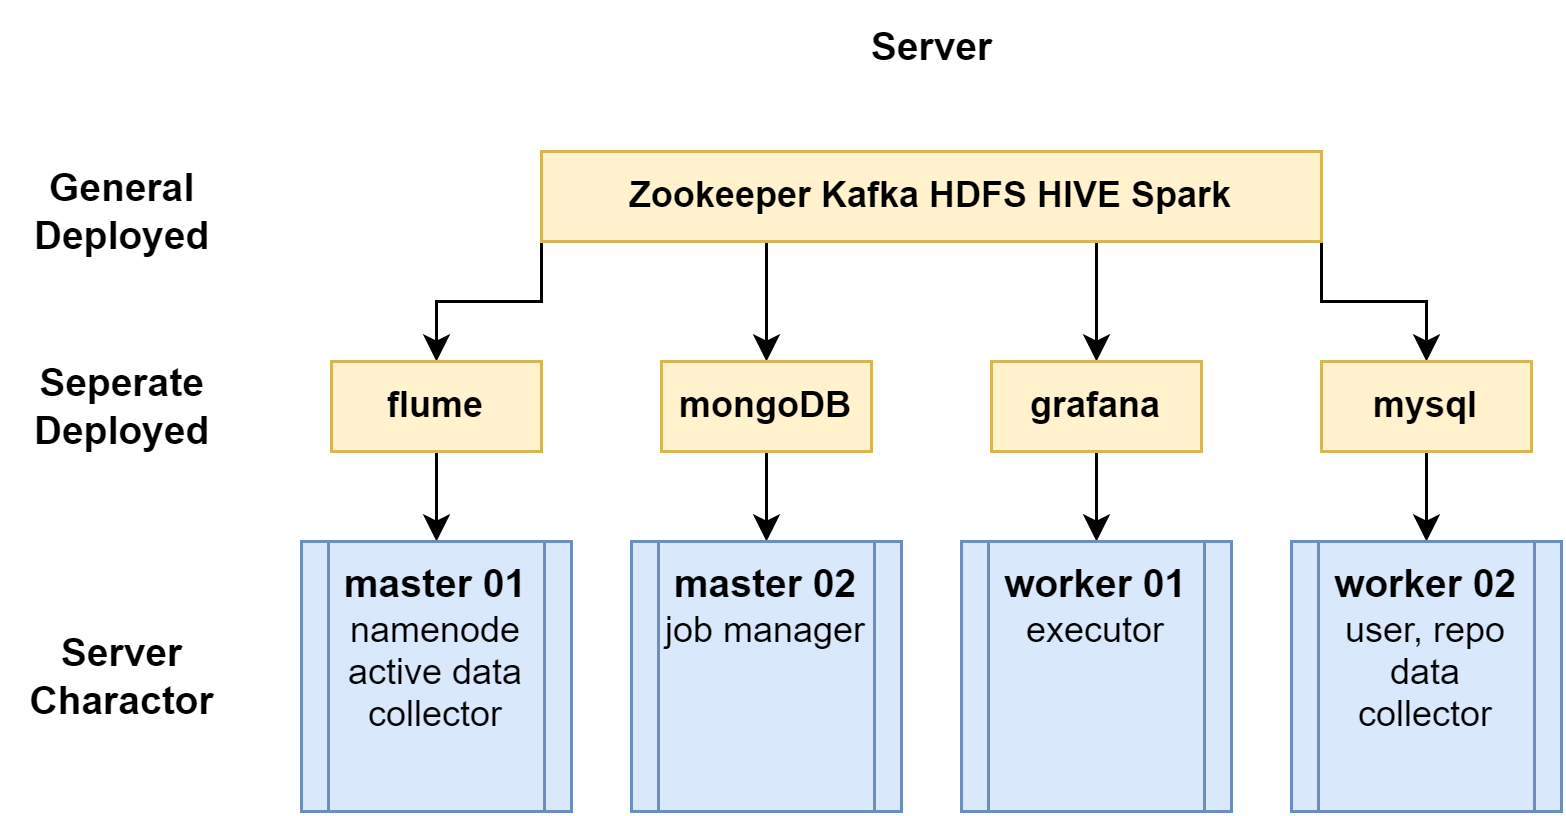
\includegraphics[width=0.5\textwidth]{./pic/deploy.png}
    \caption{A figure show the deployment of the system}
    \label{fig:deploy}
\end{figure}

Balance the server workload so that the cluster can perform at its best. Therefore, it is important to plan the placement of components. Below are the locations of the different components on the server and their basic functionality.


For the entire analysis system we use the following components. Here we briefly introduce these components:

\begin{enumerate}
    \item \textbf{Zookeeper}: ZooKeeper is a centralized service for maintaining configuration information, naming, providing distributed synchronization, and providing group services.[1] https://zookeeper.apache.org/
    \item \textbf{Kafka}: message queue, which temporarily stores data and sends it downstream. It is the data source and key part of subsequent data stream processing.
    \item \textbf{Hadoop}: Hadoop includes HDFS, Yarn and MapReduce. HDFS is the main storage place where we store data. HDFS is deployed on each server. Use Yarn as a resource manager. The resource manager is deployed on master02.
    \item \textbf{Hive}: Hive data is stored in HDFS. The hive engine is very inefficient, so only use hive as storage and data management on HDFS. Hive is deployed on the entire cluster.
    \item \textbf{Spark}: Spark is deployed on the entire cluster as the main component for data processing and data analysis.
    \item \textbf{MySQL}: The data of users and warehouses are stored in MySQL, and MySQL is deployed on worker02. At the same time, the hive meta store is also on MySQL.
    \item \textbf{Flume}: Track the data in the data capture folder and transfer it to Kafka. It will also transfer data from Kafka into a temporary folder in HDFS. The data capture process is deployed on worker02.
    \item \textbf{MongoDB}: MongoDB is deployed on master02 for expose the API.
    \item \textbf{Grafana}: Grafana is deployed on worker01. It’s the interface of data visualization.
\end{enumerate}




\subsection{Data Flow}

\begin{figure}[H]
    \centering
    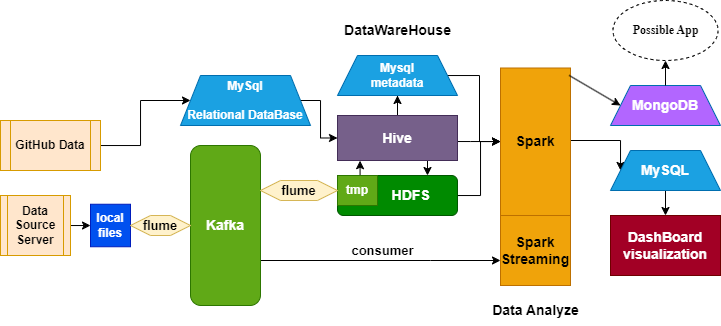
\includegraphics[width=0.5\textwidth]{./pic/dataflow.png}
    \caption{A figure shows the data flow of the system}
    \label{fig:dataflow}
\end{figure}


The server structure section introduces the general data flow direction, and here is a detailed description of the data flow in the overall analysis system.

\paragraph*{1. Data source}
The data sources are divided into two parts.
The first part is GitHub user behavior log information. The source of this part of the information is the GitHub Archive website, from which one hour of data can be obtained every hour. We temporarily store the acquired data in a folder of worker02 through the Python program for subsequent data capture.
The second part is GitHub user personal information and repo information. The source of this part of information is the official server API provided by GitHub. We use Python crawlers to obtain user and repo data through these APIs and write them into the MySQL database, and the database keeps updating these data.

\paragraph*{2. Data transmission channel}
Data transmission channels mainly include flume and kafka.
The obtained log information tracks the file information through Flume, and transmits the continuously arriving data content to Kafka. Kafka internal data can be used by spark streaming through consumer. At the same time, Kafka and HDFS are connected through flume. The data accumulated in Kafka is consumed in batches and stored in the temporary folder of HDFS.

\paragraph*{3. Data load}
MySQL memory has continuously updated user and repository information. The temporary folder of HDFS has continuously added log information. We incrementally synchronize MySQL data to Hive through the spark program. Build it into a Hive table. The data of the Hive table is stored in HDFS.
At the same time, the log information in the temporary folder is imported through Hive, and the original data is transferred to Hive for subsequent use by using the JSON serde parsing package.

\paragraph*{4. Data Warehouse Construction}
Build a data warehouse based on the acquired data. The details will be explained later.

\paragraph*{5. Data analysis}
Spark directly extracts the data in the Hive data warehouse to analyze various indicators through the built data warehouse, and writes the analyzed results into multiple different databases for different purposes:
Write to MySQL for subsequent data display.
Write to MongoDB to expose Api externally.
Write to Hive for historical data storage.
Spark streaming directly obtains data through kafka for real-time data processing, so as to obtain updated and fast real-time data display.




\subsection{Data Warehouse Construction}



\subsubsection{Modeling}


\begin{figure}[H]
    \centering
    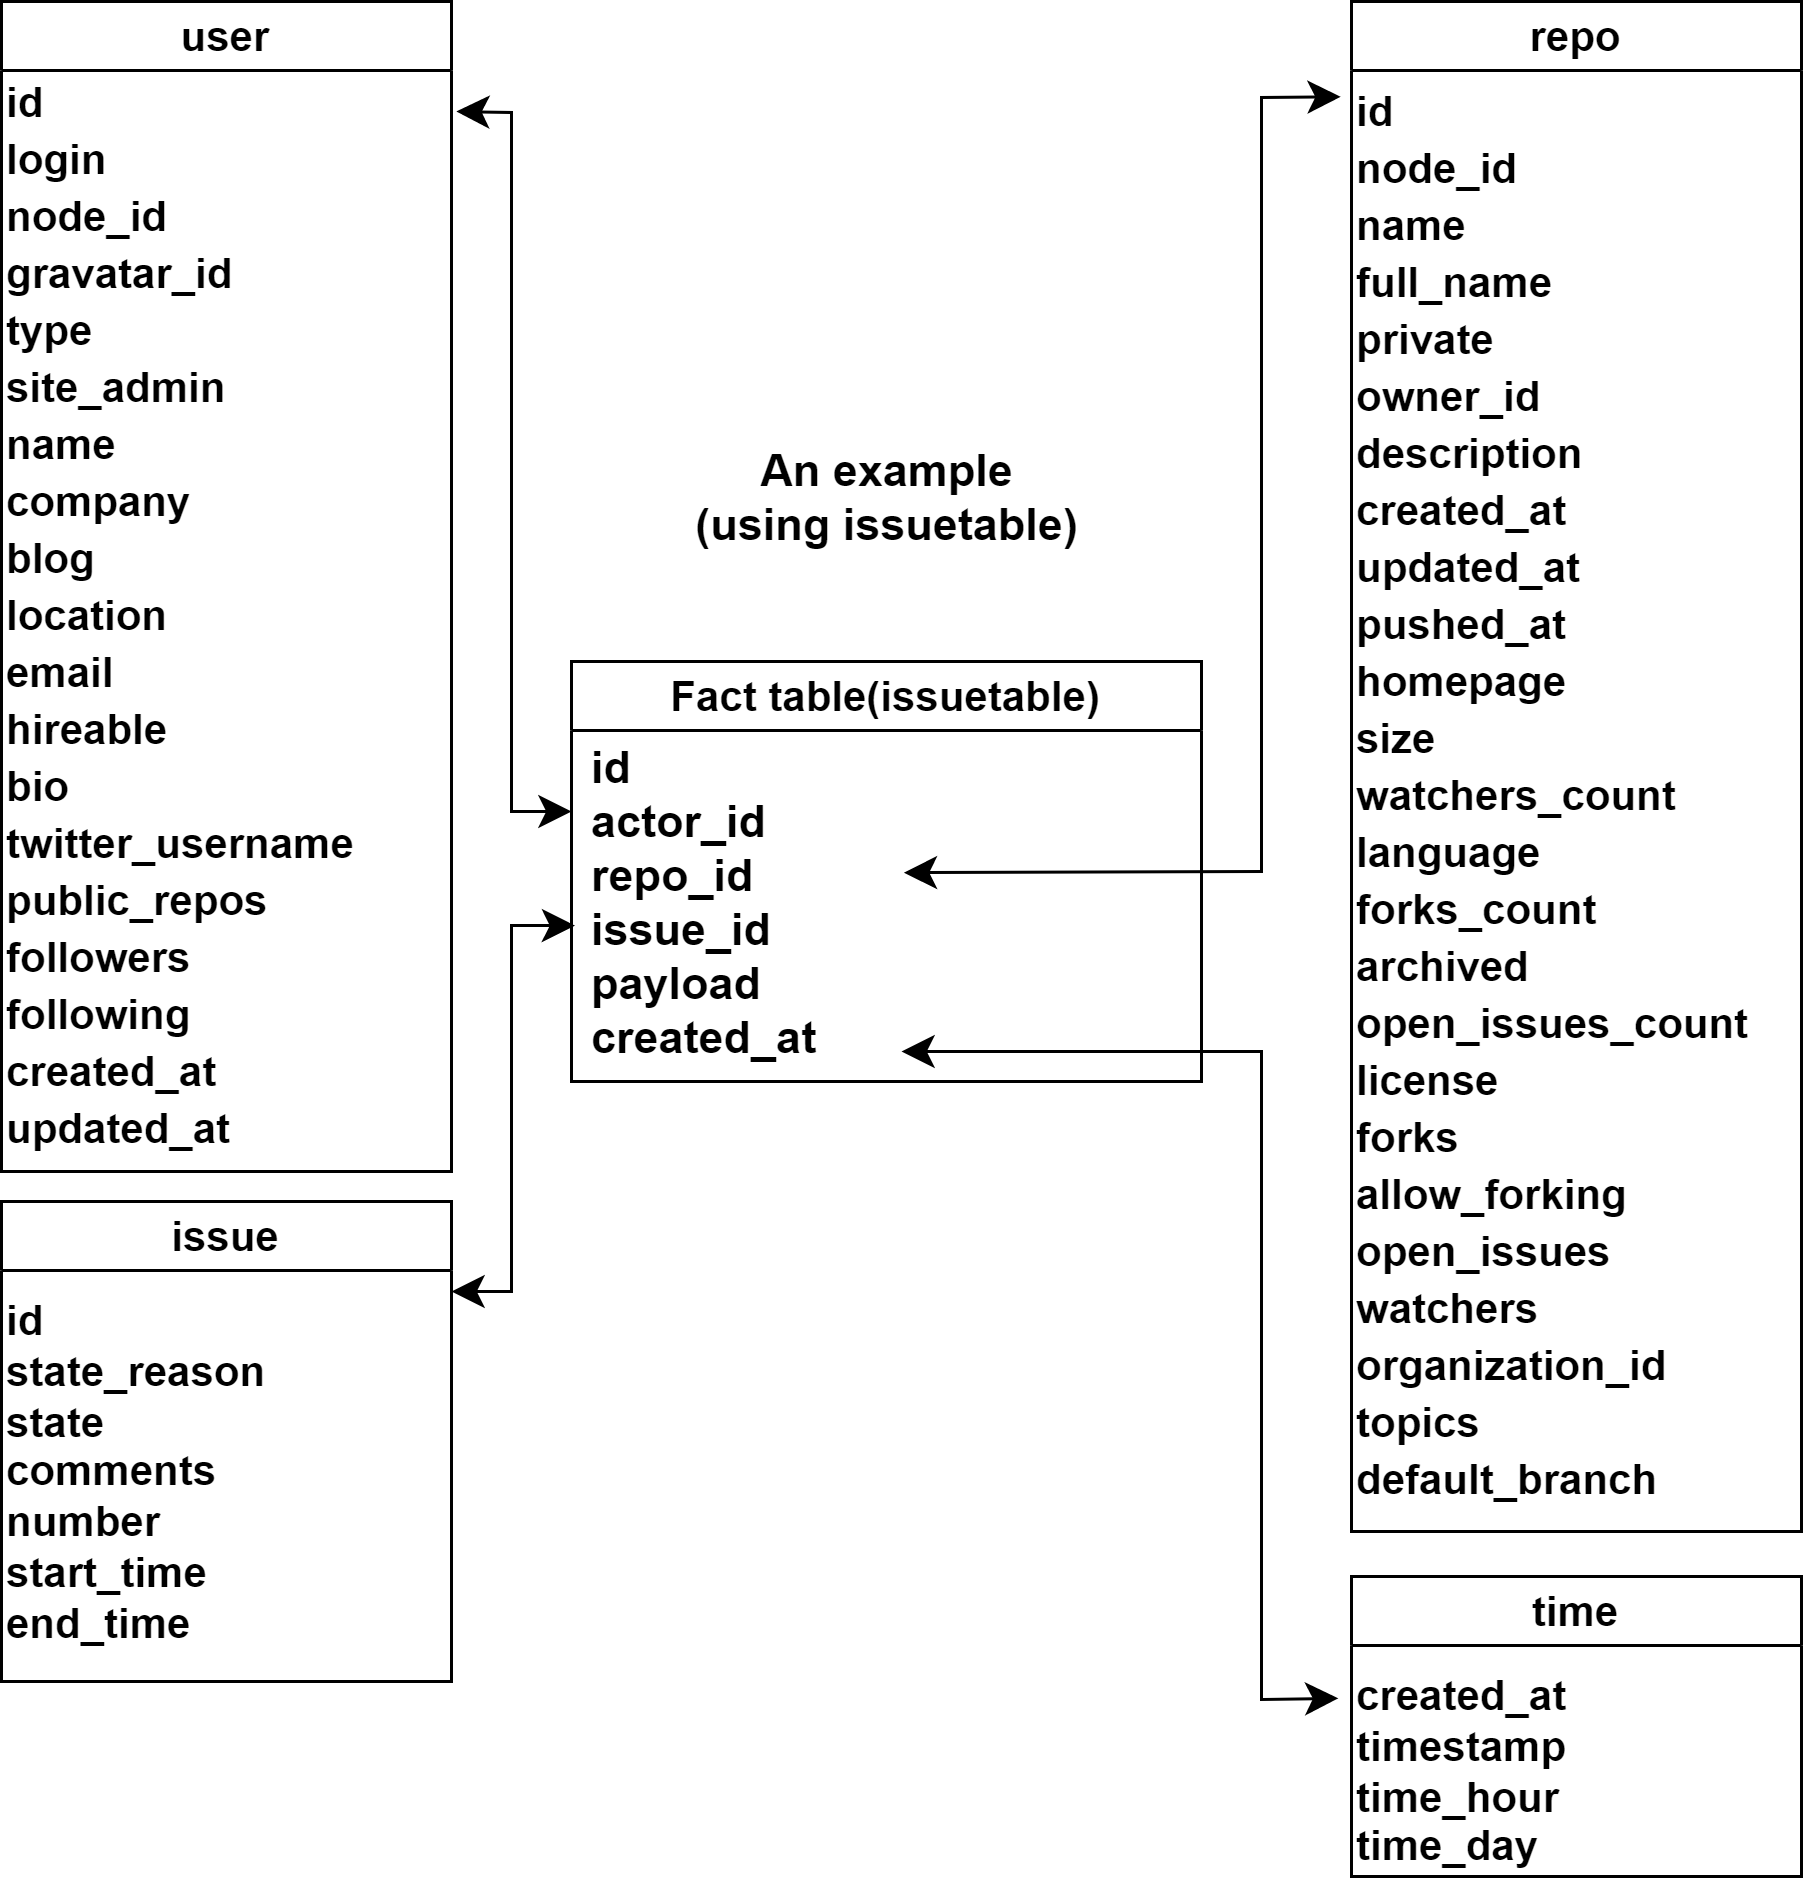
\includegraphics[width=0.5\textwidth]{./pic/tables.png}
    \caption{A figure shows the schema of the data warehouse}
    \label{fig:tables}
\end{figure}



The basic structure of data warehouse modeling adopts constellation model. There is a star schema for each transaction table, and different transaction tables share the same dimension table to form the entire constellation model.

Data granularity selection: The log data itself comes from every operation of GitHub users, and there is a corresponding time record for each operation. Since the data is acquired in one batch at the same time during the data acquisition process, the time granularity is selected to be as fine as 1 hour.

Determination of dimension table and transaction table: the dimension table adopts four dimensions of user, repo, issue and time, and the transaction table is divided into 8 types of transaction tables, such as create, delete, pull, and push, according to the different behavior of users.




\subsubsection{Hierarchy}


\begin{figure}[H]
    \centering
    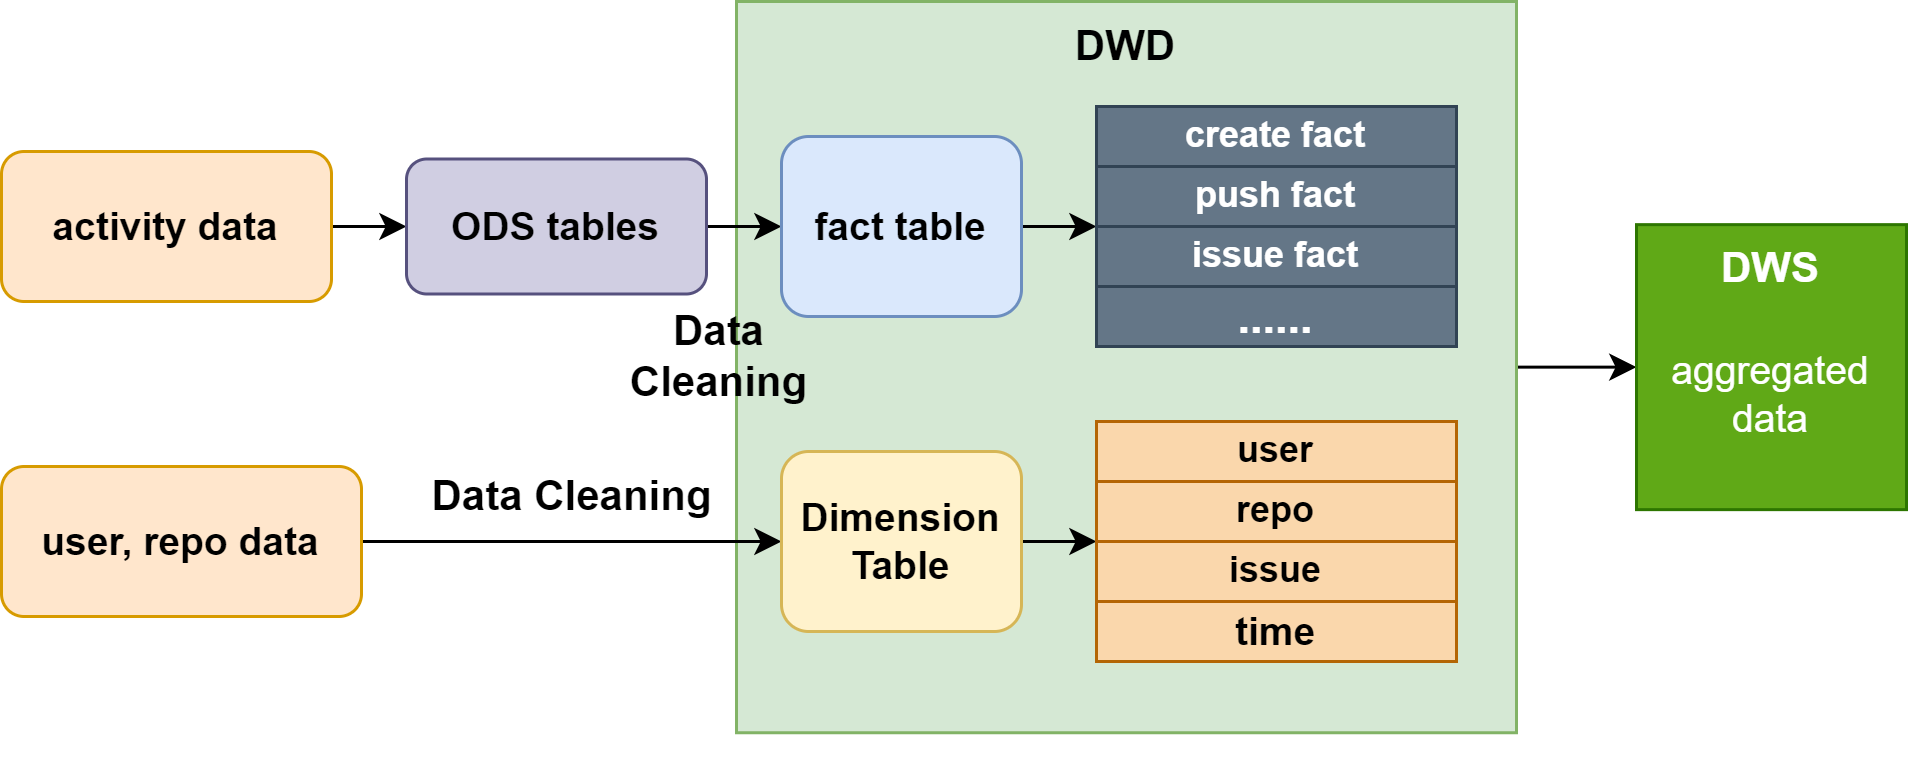
\includegraphics[width=0.5\textwidth]{./pic/warehouse.png}
    \caption{A figure shows details of the data warehouse}
    \label{fig:}
\end{figure}

\begin{itemize}
    \item \textbf{ODS layer}: When data is imported into Hive through the HDFS temporary data storage folder, the initial ODS layer table is formed. The ODS table stores the initial data without any data cleaning and processing.
    \item \textbf{DWD layer}: The data of the DWD layer comes from ODS and MySQL. The first is the transaction table. The data in the ODS layer is cleaned and preprocessed through the Spark program, invalid data and useless attributes are removed, valid information is screened, the retained content is determined, and the data is sorted out. Finally, different styles of data tables are constructed according to the type of data. These tables are all derived from the original user activity data of the ODS layer and the transaction tables are finally constructed. Then there are dimension tables. The specific information of the dimension table has already been determined, and there is synchronously updated data in MySQL. For the synchronization update process of MySQL, incremental synchronization will be performed in Hive to import data. Therefore, historical information of users and repo data will also be stored in Hive.
    \item \textbf{DWS layer}: Aggregate data at different levels for existing historical data information. After data aggregation for different time spans, the snapshot information is saved in the Hive data table to form various basic indicator results.
    \item \textbf{Data display}: Spark will use these basic indicators for analysis and processing, and transfer the results to the MySQL database for data display.
\end{itemize}







\section{Data Analysis}

After the data was aggregated into the warehouse, we collected various tables with good structural characteristics, and based on this, we used spark to further get some useful analysis results, which will also be stored into MySQL and MongoDB for further use.


Because user data on github is sparse, which means activity is not continuous and there isn't a strong pattern of activity, so there is no obvious causal relationship between attributes. For example, a large number of followers does not mean that he has a popular warehouse with a large number of stars, nor does the number of starts in a warehouse increase with the increase of fork. In other words, they reflect the same trend of users and warehouses - Degree of popularity, so we need huge dataset to analyze a very long time period to find a hidden weak pattern. Based on this, we only finished some simple aggregation and visualization of the data.


\subsection{Aggregation}





\subsection{Visualization}
We used grafana to visualize the results stored in Mysql, which are produced by spark. 

\section{summary}


\section{Summary}

Based on Github's activity data, we will use Spark and corresponding tools to construct a real-time processing framework, which will be deployed on a cloud cluster. We will show more comprehensive analysis of Github by using this framework.



% \section*{Acknowledgment}

% The contribution of our team members are as follows:



\begin{thebibliography}{00}
\bibitem{gha}https://www.gharchive.org/
\bibitem{ghapi}https://docs.github.com/en/rest?apiVersion=2022-11-28
\bibitem{ghtrending}https://github.com/trending
\bibitem{ghtopics}https://github.com/topics
\end{thebibliography}

\appendices

\section{Github REST API Example}
\label{a-ghrest}

There are some API's calling examples.


\subsection{Get All Followers of a User}

\begin{minted}[breaklines,breakautoindent,mathescape,linenos,numbersep=1pt,frame=lines,framesep=2mm,fontsize=\footnotesize,baselinestretch =1,style=emacs]{python}
https://api.github.com/users/mateiz/followers
\end{minted}


\begin{minted}[breaklines,breakautoindent,mathescape,linenos,numbersep=1pt,frame=lines,framesep=2mm,fontsize=\footnotesize,baselinestretch =1,style=emacs]{json}
    [
        {
            "login": "bennettandrews",
            "id": 1143,
            "node_id": "MDQ6VXNlcjExNDM=",
            "avatar_url": "https://avatars.githubusercontent.com/u/1143?v=4",
            "gravatar_id": "",
            "url": "https://api.github.com/users/bennettandrews",
            "html_url": "https://github.com/bennettandrews",
            ...
        },
        ...
    ]
\end{minted}


\subsection{Get Repository's Detailed Information}

\begin{minted}[breaklines,breakautoindent,mathescape,linenos,numbersep=1pt,frame=lines,framesep=2mm,fontsize=\footnotesize,baselinestretch =1,style=emacs]{python}
https://api.github.com/repos/apache/spark
\end{minted}


\begin{minted}[breaklines,breakautoindent,mathescape,linenos,numbersep=1pt,frame=lines,framesep=2mm,fontsize=\footnotesize,baselinestretch =1,style=emacs]{json}
    {
        "id": 17165658,
        "node_id": "MDEwOlJlcG9zaXRvcnkxNzE2NTY1OA==",
        "name": "spark",
        "full_name": "apache/spark",
        "private": false,
        "owner": {
            "login": "apache",
            "id": 47359,
            ...
        }
        ...
    }
\end{minted}



\subsection{Get All Commits of a Repository}

\begin{minted}[breaklines,breakautoindent,mathescape,linenos,numbersep=1pt,frame=lines,framesep=2mm,fontsize=\footnotesize,baselinestretch =1,style=emacs]{python}
https://api.github.com/repos/apache/spark/commits
\end{minted}


\begin{minted}[breaklines,breakautoindent,mathescape,linenos,numbersep=1pt,frame=lines,framesep=2mm,fontsize=\footnotesize,baselinestretch =1,style=emacs]{json}
    [
        {
            "sha": "0fde146e8676ab9a4aeafebb1684eb7a44660524",

            "commit": {
                "author": {
                    "name": "Juliusz Sompolski",
                    "email": "julek@databricks.com",
                    "date": "2023-03-24T01:56:26Z"
                },
                "committer": {
                    "name": "Hyukjin Kwon",
                    "email": "gurwls223@apache.org",
                    "date": "2023-03-24T01:56:26Z"
                },
                "message": "...",
                "tree": {
                    "sha": "308faa10a134402eb4e0796c54b4e4dd000fc7dc"
                },
                ...
            },
            "author": {
                "login": "juliuszsompolski",
                "id": 25019163,
                "node_id": "MDQ6VXNlcjI1MDE5MTYz",
                ...
            },
            "committer": {
                "login": "HyukjinKwon",
                "id": 6477701,
                ...
            },
            "parents": [{}]
        },
        ...
    ]
\end{minted}




\section{GH Archive}
\label{a-gha}

One single json record from the GH Archive.

\begin{minted}[breaklines,breakautoindent,mathescape,linenos,numbersep=1pt,frame=lines,framesep=2mm,fontsize=\footnotesize,baselinestretch =1,style=emacs]{json}
    [
        {
            "id": "2489651051",
            "type": "PushEvent",
            "actor": {
                "id": 3854017,
                "login": "rspt",
                "gravatar_id": "",
                "url": "https://api.github.com/users/rspt",
                "avatar_url": "https://avatars.githubusercontent.com/u/3854017?"
            },
            "repo": {
                "id": 28671719,
                "name": "rspt/rspt-theme",
                "url": "https://api.github.com/repos/rspt/rspt-theme"
            },
            "payload": {
                "push_id": 536863970,
                "size": 1,
                "distinct_size": 1,
                "ref": "refs/heads/master",
                "head": "6b089eb4a43f728f0a594388092f480f2ecacfcd",
                "before": "437c03652caa0bc4a7554b18d5c0a394c2f3d326",
                "commits": [
                    {
                        "sha": "6b089eb4a43f728f0a594388092f480f2ecacfcd",
                        "author": {
                            "email": "5c682c2d1ec4073e277f9ba9f4bdf07e5794dabe@rspt.ch",
                            "name": "rspt"
                        },
                        "message": "Fix main header height on mobile",
                        "distinct": true
                    }
                ]
            },
            "public": true,
            "created_at": "2015-01-01T15:00:01Z"
        },
        ...
    ]
\end{minted}




\end{document}
